\begin{figure}[htbp]\centering
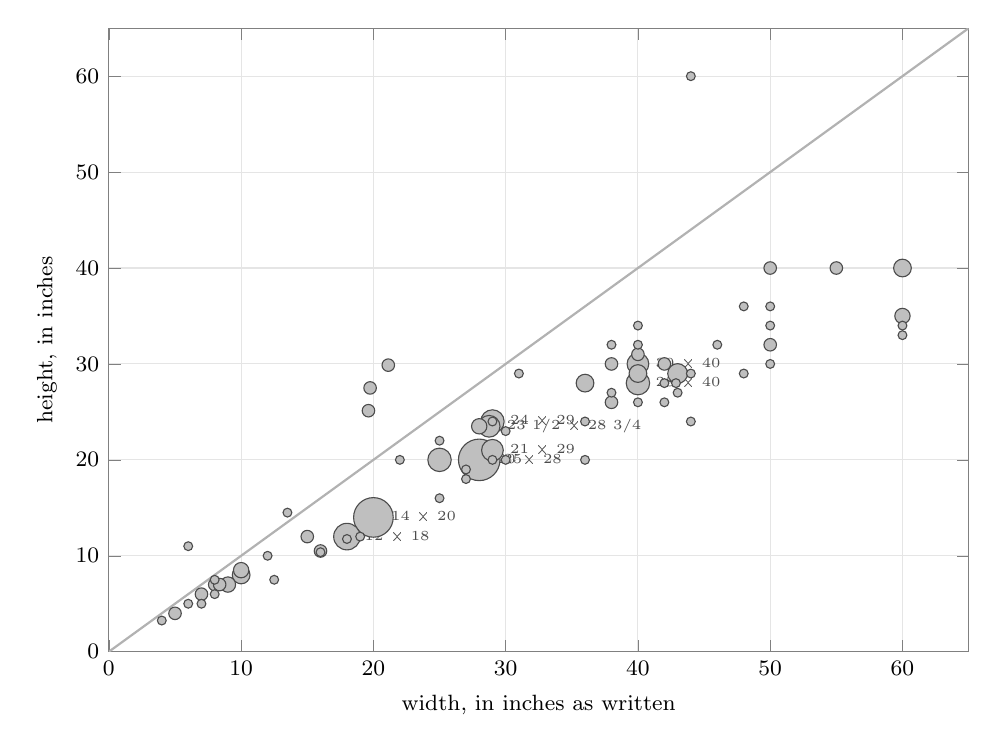
\begin{tikzpicture}
\begin{axis}[width=12.5cm,height=9.5cm,xmin=0,xmax=65,ymin=0,ymax=65,xlabel={width, in inches as written},ylabel={height, in inches},grid=both,grid style={black!10},tick label style={font=\footnotesize},label style={font=\footnotesize},axis line style={black!50}]
\addplot[black!30,thick,domain=0:65] {x};
\addplot[scatter,only marks,mark=*,scatter/use mapped color={draw=black!70,fill=black!25},visualization depends on={\thisrow{n} \as \n},scatter/@pre marker code/.append style={/tikz/mark size={sqrt(\n)*1.6pt}},point meta=\thisrow{n}] table[x=w,y=h] {
w h n
28 20 22
20 14 20
18 12 9
25 20 7
29 24 7
40 28 7
29 21 6
28.75 23.5 6
40 30 6
43 29 5
10 8 4
36 28 4
40 29 4
60 40 4
9 7 3
10 8.5 3
28 23.5 3
60 35 3
5 4 2
7 6 2
8 7 2
8.375 7 2
16 10.5 2
15 12 2
19.625 25.125 2
19.75 27.5 2
21.125 29.875 2
38 26 2
38 30 2
40 31 2
42 30 2
50 32 2
50 40 2
55 40 2
4 3.25 1
6 5 1
7 5 1
8 6 1
8 7.5 1
6 11 1
12.5 7.5 1
12 10 1
16 10.375 1
13.5 14.5 1
18 11.75 1
19 12 1
25 16 1
22 20 1
27 18 1
27 19 1
25 22 1
29 20 1
30 20 1
30 23 1
29 24 1
36 20 1
36 24 1
31 29 1
38 27 1
40 26 1
44 24 1
42 26 1
43 27 1
42 28 1
42.875 28 1
38 32 1
44 29 1
40 32 1
40 34 1
48 29 1
46 32 1
50 30 1
50 34 1
48 36 1
50 36 1
60 33 1
60 34 1
44 60 1
};
\node[font=\tiny,anchor=west,text=black!70] at (axis cs:28.6,20) {20 × 28};
\node[font=\tiny,anchor=west,text=black!70] at (axis cs:20.6,14) {14 × 20};
\node[font=\tiny,anchor=west,text=black!70] at (axis cs:18.6,12) {12 × 18};
\node[font=\tiny,anchor=west,text=black!70] at (axis cs:25.6,20) {20 × 25};
\node[font=\tiny,anchor=west,text=black!70] at (axis cs:29.6,24) {24 × 29};
\node[font=\tiny,anchor=west,text=black!70] at (axis cs:40.6,28) {28 × 40};
\node[font=\tiny,anchor=west,text=black!70] at (axis cs:29.6,21) {21 × 29};
\node[font=\tiny,anchor=west,text=black!70] at (axis cs:29.35,23.5) {23 1/2 × 28 3/4};
\node[font=\tiny,anchor=west,text=black!70] at (axis cs:40.6,30) {30 × 40};
\end{axis}
\end{tikzpicture}
\caption{Every format, plotted: width across, height up, one dot to a format and its area standing for how many works were made at it, 78 formats from 199 work headings that state a size. The diagonal is where a picture would be square; 190 of the 199 works lie below it, 9 above, none on it. The etching plates are in the corner, the watercolour sheets through the middle, the late oils at the top right. After the Technique tab of hopper.commutator.io. Drawn by Claude Fable~5.1, 13 September 2026, from \texttt{formats.json} (undated).}\label{fig:scatter}
\end{figure}
